%
% Copyright 2018 Markus Borg, Lund University
%
% This work is licensed under a Creative Commons Attribution-ShareAlike 4.0 International License.
% See http://creativecommons.org/licenses/by-sa/4.0/
%
% The dodument is based on a LaTeX template developed by Jean-Philippe Eisenbarth
% https://github.com/jpeisenbarth/SRS-Tex
%
\documentclass{scrreprt}
\usepackage{graphicx}
\usepackage{listings}
\usepackage{underscore}
\usepackage[bookmarks=true]{hyperref}
\usepackage[utf8]{inputenc}
\usepackage[english]{babel}
\hypersetup{
    bookmarks=false,    % show bookmarks bar?
    pdftitle={Lab 4},    % title
    pdfauthor={Markus Borg},                     % author
    pdfsubject={TeX and LaTeX},                        % subject of the document
    pdfkeywords={TeX, LaTeX, graphics, images}, % list of keywords
    colorlinks=true,       % false: boxed links; true: colored links
    linkcolor=blue,       % color of internal links
    citecolor=black,       % color of links to bibliography
    filecolor=black,        % color of file links
    urlcolor=purple,        % color of external links
    linktoc=page            % only page is linked
}%
\def\myversion{0.3 }
\date{}
%\title
\usepackage{hyperref}
\begin{document}

\begin{flushright}
    \rule{16cm}{5pt}\vskip1cm
    \begin{bfseries}
    	\LARGE{ETSA02-ADM-LAB4}\\
    	\vspace{1.5cm}
        \Huge{Lab 4}\\
        \vspace{0.5cm}
        Code coverage testing,\\
        \vspace{0.5cm}
        static code anaysis,\\
        \vspace{0.5cm}
        and Javadoc\\
        \vspace{1.5cm}
        \LARGE{Version \myversion approved}\\
        \vspace{1.5cm}
        Prepared by Markus Borg\\
        %\vspace{1.5cm}
        Dept. of Computer Science, Lund University\\
        \vspace{1.5cm}
        \today\\
    \end{bfseries}
\end{flushright}

%\tableofcontents

\chapter*{Revision History}

\begin{center}
    \begin{tabular}{|c|c|c|c|}
        \hline
	    Name & Date & Reason For Changes & Version\\
        \hline
	    Markus Borg & 2018-04-18 & Initial structure. & 0.1\\
        \hline
        Markus Borg & 2018-04-21 & Added EclEmma, SpotBugs, and SonarLint. & 0.2\\
        \hline
        Markus Borg & 2018-04-22 & Complete draft, ready for internal review. & 0.3\\
        \hline
        Markus Borg & 2018-04-24 & Updated after internal review, ready for lab. & 1.0\\
        \hline
    \end{tabular}
\end{center}

\chapter{Introduction}
Lab 4 focuses on source code quality assurance for Basic Melee Bot. High-quality source code is your best approach to decrease the chances of releasing a robot with bugs, and it also greatly improves the maintainability of the product. First, you will add code coverage measurements to your existing suite of unit tests. Second, you will explore two established tools for static code analysis. Finally, you will generate Javadoc for Basic Melee Bot, i.e., the de facto industry standard for documenting Java classes. More specifically, Lab 4 covers the following:

\begin{itemize}
\item Code coverage testing with EclEmma
\item Static code analysis with SpotBugs and SonarLint
\item Generating Javadoc from Eclipse
\end{itemize}

\chapter{Before the lab}
If you still have the Java project from either Lab 2 or Lab 3 in your workspace, then you have everything you need for Lab 4. The source code used in Lab 4 is Basic Melee Bot and its accompanying unit test suite (introduced in Lab 2, but available also in Lab 3). On the other hand, if you are now comfortable with downloading and importing source code from GitHub, you can of course download the latest version. If you want the latest code, Lab 4 has been prepared in the course repository on GitHub:\\https://github.com/lunduniversity/introsofteng\\\\
The same instructions as from Lab 2 and Lab3 apply: if you have already cloned the repository, pull the latest source code to make sure you work with the latest version. If you prefer downloading the code, instead click the button presented in Figure~\ref{fig:github} and choose ``Download ZIP''. Once downloaded, locate the files you need for Lab 4. The files are in the folder introsofteng-master/labs/lab4/src, and its subfolder: `test'. Rewatch the video ``Lab2_download.avi'' on Google Drive (ETSA02 Everyone/Labs) if you need support.

To prepare for the lab session, please make sure you can execute a unit test suite for Basic Melee Bot. Then have a look at the following pages:
\begin{itemize}
\item Code coverage (skip ``Modified condition/decision coverage'' and onwards)\\-- https://en.wikipedia.org/wiki/Code_coverage
\item EclEmma homepage (browse the page to get a high-level understanding) \\-- http://www.eclemma.org/
\item Coverage counters in JaCoCo (library used by eclEmma) \\-- http://www.eclemma.org/jacoco/trunk/doc/counters.html
\item Static code analysis (skip ``Formal methods'') \\-- https://en.wikipedia.org/wiki/Static_program_analysis
\item SpotBugs homepage (browse the page to get a high-level understanding) \\-- https://spotbugs.github.io/
\item SonarLint homepage (browse the page to get a high-level understanding) \\-- https://www.sonarlint.org/
\item Javadoc document generator \\-- https://en.wikipedia.org/wiki/Javadoc
\end{itemize}

\chapter{At the lab} \label{sec:atlab}
In Lab 4, you will learn to download open source tools from the big Eclipse ecosystem through Eclipse Marketplace. You reach Eclipse Marketplace directly from your Eclipse installation: Select ``Eclipse Marketplace...'' from the Help menu.

\section{Code coverage with EclEmma}
First, you will work with code coverage testing. Search for EclEmma on Eclipse Marketplace, and install the latest version: EclEmma Java Code Coverage 3.0.1. EclEmma introduces a new run option in Eclipse, beyond ``Run as...'' and ``Debug as...''. The new run option is called ``Coverage as...''. The eclEmma ``Coverage view'' automatically appears when a new coverage session is added or can manually be opened from the Window $\rightarrow$ Show View menu in the Java category. 

The coverage view shows code coverage summaries for the active session. Individual columns in the view contain the following numbers for the active session, always summarizing the child elements of the respective Java element:

\begin{itemize}
\item Coverage ratio
\item Items covered
\item Items not covered
\item Total items
\end{itemize}

The elements may be sorted in ascending or descending order by clicking the respective column header. Double-clicking an element opens its declaration in an editor with highlighted source code. Figure~\ref{fig:eclemma} shows an example of the coverage view, and how to switch between different coverage metrics, i.e., instruction counters, branch counters, line counters, method counters, type counters, and complexity. Not that you can also remove the coverage annotation from the coverage view by clicking the cross icons.

\begin{figure}
\centering
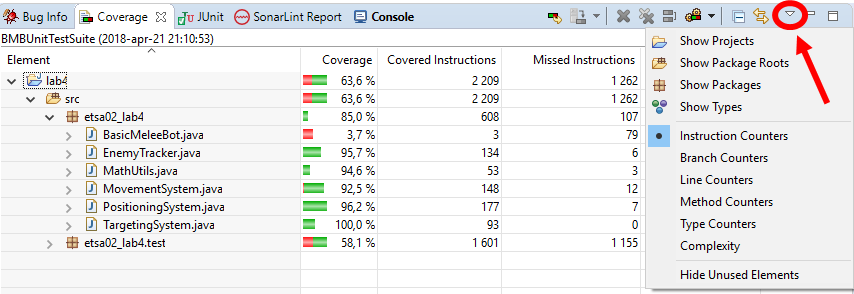
\includegraphics[width=0.99\textwidth]{figures/EclEmma.png}
\caption{The coverage view in EclEmma. The circle shows where to switch coverage metric.}
\label{fig:eclemma}
\end{figure}

Now it is time to perform a code coverage measurement of Basic Melee Bot to analyze to what extent the unit test suite covers the source code of the robot. In the ``Package Explorer'' in Eclipse, right click the unit test suite in your Java project (``AllBasicMeleeBotUnitTests.java'' if working with Lab 2, otherwise ``BMBUnitTestSuite.java'') and choose ``Coverage as'' $\rightarrow$ JUnit Test. The unit test suite will run as before, but you will also get coverage measurements. Explore the results in the EclEmma coverage view (skip coverage of the classes in the test package). Double click on elements in the coverage view to navigate to color coded source code, for which green = covered, yellow = partly covered, and red = not covered. Then try to answer the following questions:
\begin{itemize}
\item What is the total instruction coverage?
\item Which classes have the highest instruction coverage? Why?
\item Which classes have the lowest instruction coverage? Why?
\item What do the other coverage metrics reveal?   
\item Would you recommend us to add more unit tests to Basic Melee Bot?
\end{itemize}

\section{Static code analysis with SpotBugs and SonarLint}
The second part of Lab 4 is about static code analysis tools. Search for SpotBugs on Eclipse Marketplace, and install the latest version: SpotBugs Eclipse plugin 3.1.2. While you are at it, search also for SonarLint, and install the latest version: SonarLint 3.4.

Run SpotBugs by right clicking your Java project in Package Explorer and select SpotBugs $\rightarrow$ Find Bugs as shown in Figure~\ref{fig:spotbugs}. SpotBugs comes with its own Eclipse ``Perspective'' (a set and layout of views in the Workbench window). If the perspective has not opened yet, open it in the Window menu $\rightarrow$ Perspective $\rightarrow$ Open Perspective $\rightarrow$ Other... and select ``SpotBugs'' in the resulting dialog window.

In the SpotBugs perspective you have a view called ``Bug Explorer'', analogous to the well-known ``Package Explorer''. Use it to identify the issue identified by SpotBugs. Right click the issue in Bug Explorer and select ``Show Bug Info'' to read more. Double click the issue in Bug Explorer to directly navigate to the corresponding line in the source code. Do you understand the issue? Can you resolve it? Sometimes you want to modify the severity level of issues that SpotBugs should report. To do so, right click your Java project and select Properties. Under SpotBugs you can configure the minimum rank for SpotBugs to report, with severities ranging from 1 to 20 -- however, the default level is already appropriate for your work in the project.

\begin{figure}
\centering
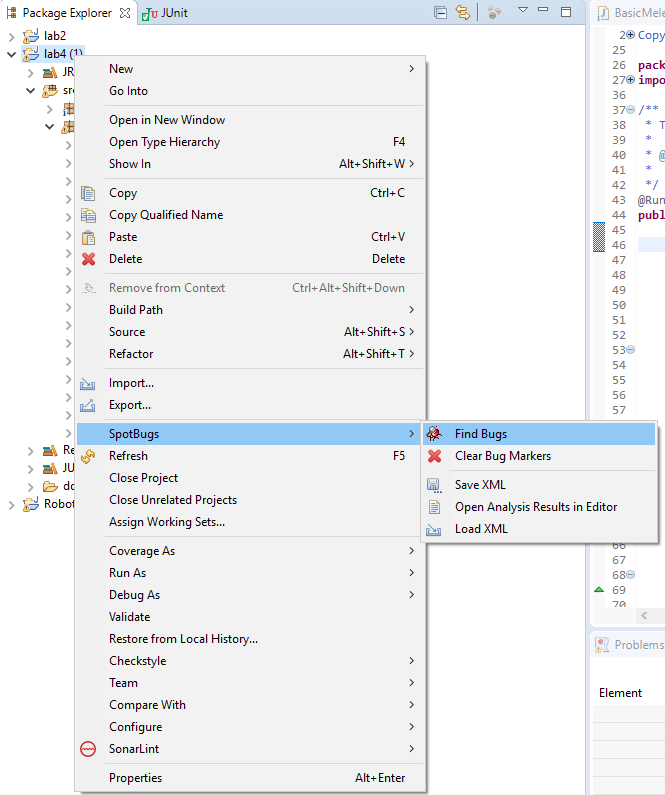
\includegraphics[width=0.75\textwidth]{figures/SpotBugs.png}
\caption{Running SpotBugs on your project.}
\label{fig:spotbugs}
\end{figure}

Run SonarLint by right clicking your Java project in Package Explorer and select SonarLint $\rightarrow$ Analyze. A dialog appears to warn you that it might take a while to complete this action, but this is no problem at all for projects as small as ours. SonarLint introduces new Eclipse views (like EclEmma). If they are not yet visible, open two of them in the Window menu $\rightarrow$ Show View $\rightarrow$ Other... and select ``SonarLint'' $\rightarrow$ ``SonarLint Report'' and ``SonarLint Rule Description'' in the resulting dialog window (cf. Figure~\ref{fig:sonarlint}). 

Investigate the output in the SonarLint Report view. Each item represents a SonarLint rule violation, and each violation has an explicit severity level. How many items are listed? How many different types of rule violations have been identified? What severity levels are represented in the report? You can read more about a rule violation by right clicking it and selecting ``Rule description''. You can also double click on any rule violation in the SonarLint Report view to navigate to the corresponding line in the source code. Can you resolve any rule violations in BasicMeleeBot to reduce the list?

\begin{figure}
\centering
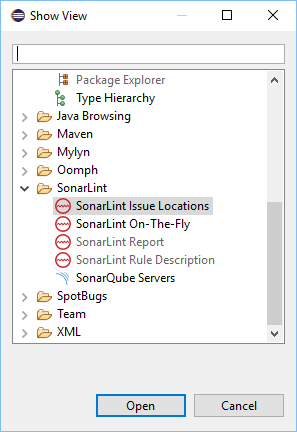
\includegraphics[width=0.33\textwidth]{figures/SonarLint.png}
\caption{Showing the SonarLint views in Eclipse.}
\label{fig:sonarlint}
\end{figure}

\section{Generating documentation using Javadoc}
The final assignment in Lab 3 is simple, but very important for high quality software: source code documentation. The de facto standard for Java documentation is Javadoc, a tool that reads structured source code comments in Java files and outputs html formatted documentation that is easy to navigate. To generate Javadoc, select ``Generate Javadoc...'' in the Project menu. The dialog presented in Figure~\ref{fig:javadoc} should appear. Select the project you want documentation for, and choose to create Javadoc for all visibility levels, i.e., select Private among the first radio buttons. The default output location is fine, just proceed through the rest of the dialog windows. When the process has completed, have a look at the generated documentation by opening ``index.html'' in the documentation output folder. Browse the documentation. Which classes are properly documented? Which should be complemented to meet the expectations on good documentation?

\begin{figure}
\centering
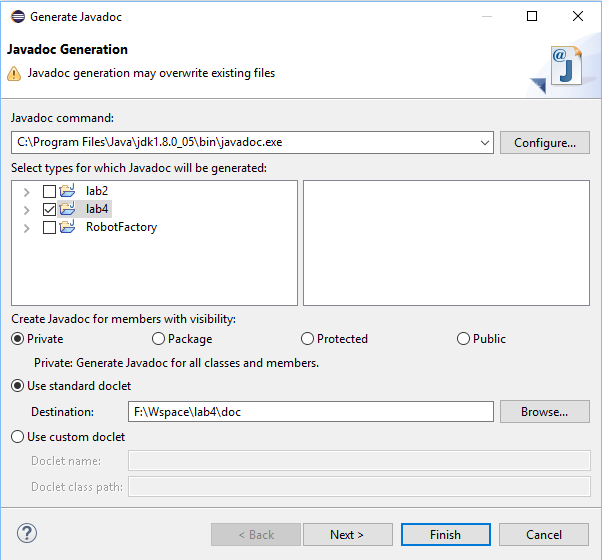
\includegraphics[width=0.75\textwidth]{figures/Javadoc.png}
\caption{Javadoc generation in Eclipse.}
\label{fig:javadoc}
\end{figure}

\chapter{After the lab}
Your group shall state a code coverage target for your unit test suite in the STS, at least instruction coverage. For the Final Release of your robot, you shall measure code coverage using EclEmma and report the outcome in the test report. Any deviations from the coverage target shall be motivated.

In the project, your group shall run the two static code analysis tools SpotBugs and SonarLint. The latest version of the STS template specifies that you shall resolve all issues identified by SpotBugs running with the default settings, but not necessarily for the test code. Your group shall report the number of issues identified by SpotBugs in the test report that is part of the Final Release. Note that any remaining SpotBugs issues shall be explained and motivated in the test report. Your group shall also run SonarLint on your source code. As specified by the STS template, the final version of the source code shall not have any remaining SonarLint rule violations of severity major or higher. Any such remaining rule violations shall be explained and motivated in the test report.

All non-customer releases in the project shall be complemented by documentation generated by Javadoc. Make sure you provide this information for the Beta Release and the Final Release. The class diagram and the Javadoc is what helps external stakeholders get an overview of your source code!
\end{document}
